\begin{exercise}{6}

\begin{subexercise}
  \begin{displaymath}
    \begin{array}{l l}
      \{ e.EmployeeId, e.LastName | & e \in employee \land \exists c \in costomer \land\\
              & \text{\texttt{COUNT}}( c.City = e.City \land e.EmployeeId =
              c.SupportRepId ) > 1 \}
    \end{array}
  \end{displaymath}
  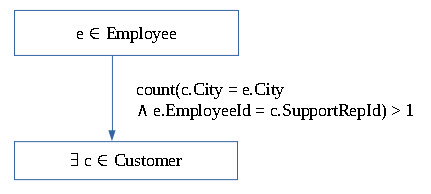
\includegraphics{ueb03/2a.jpg}
\end{subexercise}

\begin{subexercise}
  \begin{displaymath}
    \begin{array}{l l}
      \{ t.Name, t.composer | &t \in track \land \exists g\in genre \land
      \exists al\in album
      \land \exists at \in artist \land \\
            & t.AlbumId = al.AlbumId \land al.ArtistId = at.ArtistId \land
                t.composer = at.Name \land \\
            & t.GenreId = g.GenreId \land g.Name = \text{'}Rock\text{'}
        \}
    \end{array}
  \end{displaymath}
  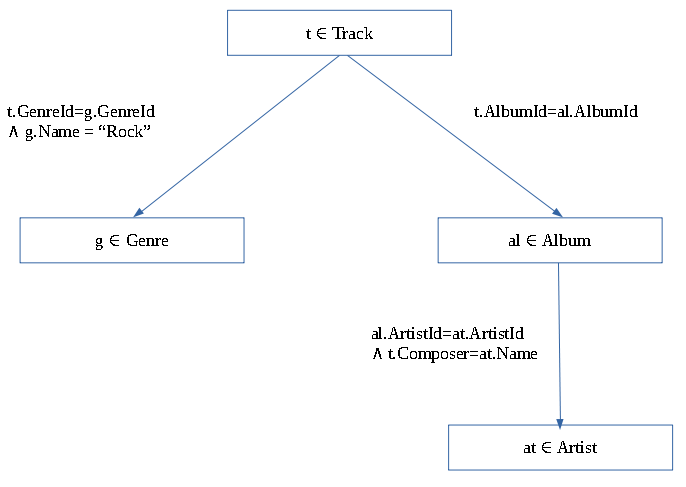
\includegraphics[width=0.7\textwidth]{ueb03/2b.png}
\end{subexercise}
\end{exercise}
